\Chapter{Felhasználói kézikönyv}

A továbbiakban szeretném bemutatni az alkalmazás használatát. Ez a kézikönyv útmutatást nyújt az egyes funkciók használatáról, lépésről lépésre, segítve a felhasználót abban, hogy hatékonyan működtesse a rendszert.

\Section{Az alkalmazás indítása}

Először is egy adatbáziskezelőt nyissunk meg és hozzunk létre egy proba28 nevű adatbázist és használjuk is azt. Ez elengedhetetlen része az alkalmazás indításának, mivel enélkül a szerveroldal el se fog indulni.\\

\begin{figure}[h]
\centering
\includegraphics[scale=1]{images/Adatbázis.png}
\caption{Adatbázis inicializálás}
\label{fig:adatbazis}
\end{figure}

Ezek után indítsuk el a backend és frontend részét az alkalmazásnak. Ehhez választhatunk bármilyen webalkalmazáshoz megfelelő fejlesztőkörnyezetet. Személy szerint a JetBrains-es termékeket javaslom, mint például az Intellij vagy a Webstorm. Fontos megjegyezni, hogy az első indításkor néhány hibaüzenet fogad minket a backend részen. Ne essünk kétségbe, mert a második indítás után ezek a hibák automatikusan el fognak tűnni. A probléma abból adódik, hogy a szerveroldal elindulásakor bizonyos műveletek próbálnak hozzáférni a már létező adatbázishoz, ami az első indításkor még nem teljesen inicializálódott. Ezért indítsuk el még egyszer a szerveroldalt.

\begin{figure}[h]
\centering
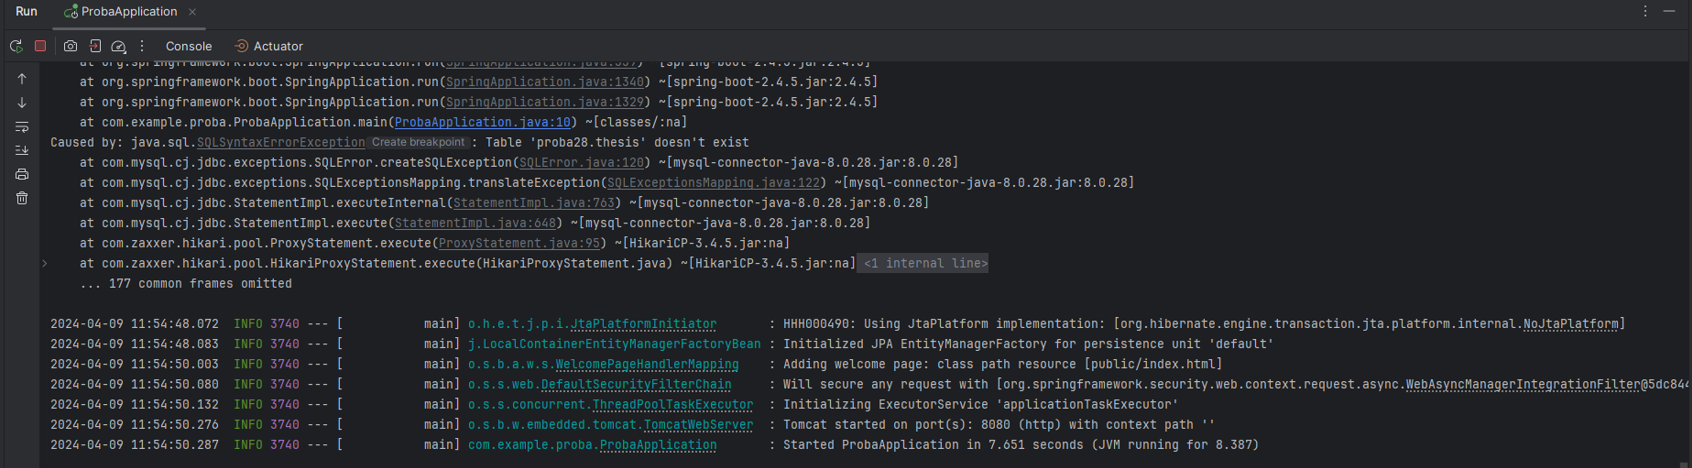
\includegraphics[width=\textwidth]{images/backend_running.png}
\caption{Backend inicializálás}
\label{fig:backend}
\end{figure}

\begin{figure}[h]
\centering
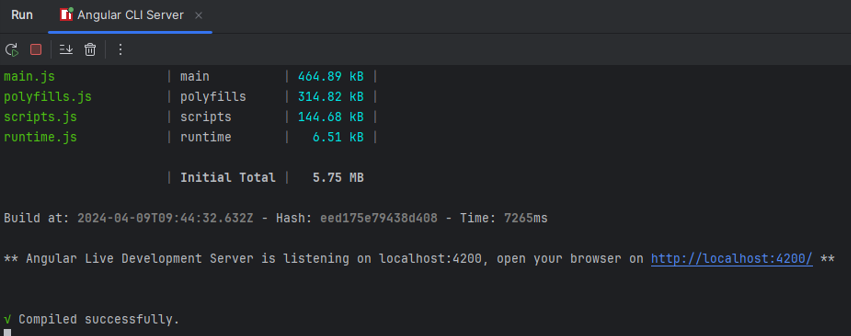
\includegraphics[width=\textwidth]{images/frontend_running.png}
\caption{Frontend inicializálás}
\label{fig:frontend}
\end{figure}
\newpage

Miután sikeresen elindítottuk az alkalmazást nyissuk meg a frontend által felkínált localhost:4200 linket.

\Section{Bejelentkezés}

Miután a linket megnyitottuk, a bejelentkező felületre érkezünk. Itt lehetőségünk van megadni a felhasználónevünket és a jelszót a belépéshez szükséges adatokként. Ha esetleg elfelejtettük a jelszavunkat, akkor az "Elfelejtett jelszó" gombra kattintva megadhatjuk a felhasználónevünket, amely egy e-mail címhez van rendelve. Ezt követően egy token-t kapunk az e-mail címünkre, amelyet a következő felugró ablakban kell használnunk. Ott kell megadnunk a felhasználónevet, a tokent és az új jelszót kétszer. A validátor segítségével ellenőrzöm, hogy a két jelszó megegyezik.

\begin{figure}[h]
\centering
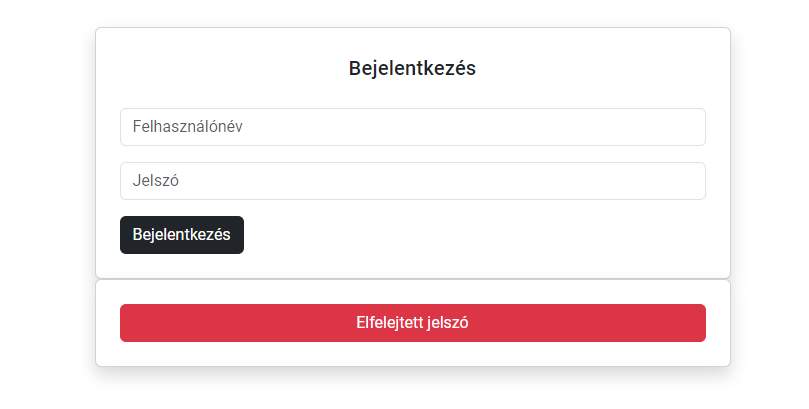
\includegraphics[width=\textwidth]{images/login.png}
\caption{Bejelentkező felület}
\label{fig:login}
\end{figure}

\newpage

A továbbiakban szeretném bemutatni a felhasználók regisztrálását, a bírálat írását és a szakdolgozatok bírálatának nyomon követését. Ezek a lapok alapvető fontosságúak az alkalmazás fő funkcionalitásainak megértéséhez és hatékony használatához. Fontosnak tartom megjegyezni, hogy bár más lapok is léteznek az alkalmazásban, melyek különböző funkciókat és információkat kínálnak, a bemutatott három lap átfogóan tartalmazza az összes implementált funkcionalitást, így biztosítva a felhasználóknak a teljes körű tudást és felhasználói élményt.



\Section{Felhasználók regisztrálása}


Az oldal lehetővé teszi a felhasználók regisztrálását, melyhez kizárólag az adminisztrátor férhet hozzá. A regisztráció során számos információt kell megadni, mint például a felhasználó titulusát (pl. dr.), születési dátumát, e-mail címét, Neptun kódját, felhasználónevet és jelszót. Emellett további adatokat is rögzíthetünk, mint a felhasználó teljes nevét, születési helyét, édesanyja leánykori nevét, munkahelyét és törzskönyvi számát. Ezek az adatok később elengedhetetlenek lehetnek a záróvizsga jegyzőkönyvéhez.\\
\\
A felhasználó szerepkörét egy legördülő listából választhatjuk ki. A helyes adatbevitelt validátorok segítik, melyek dinamikusan változnak a kiválasztott szerepkörtől függően. Ha a bíráló szerepkört választjuk, megjelenik egy extra mező, ahol a beosztást adhatjuk meg. Témavezető, jegyző és elnök esetén ezeket az adatokat legördülő listával oldottam meg.\\
\\
A felvitel gombra kattintva a rendszer egy sikeres vagy sikertelen üzenettel fogad minket, tájékoztatva arról, hogy a felhasználó sikeresen felkerült-e az adatbázisba.

\begin{figure}[h]
\centering
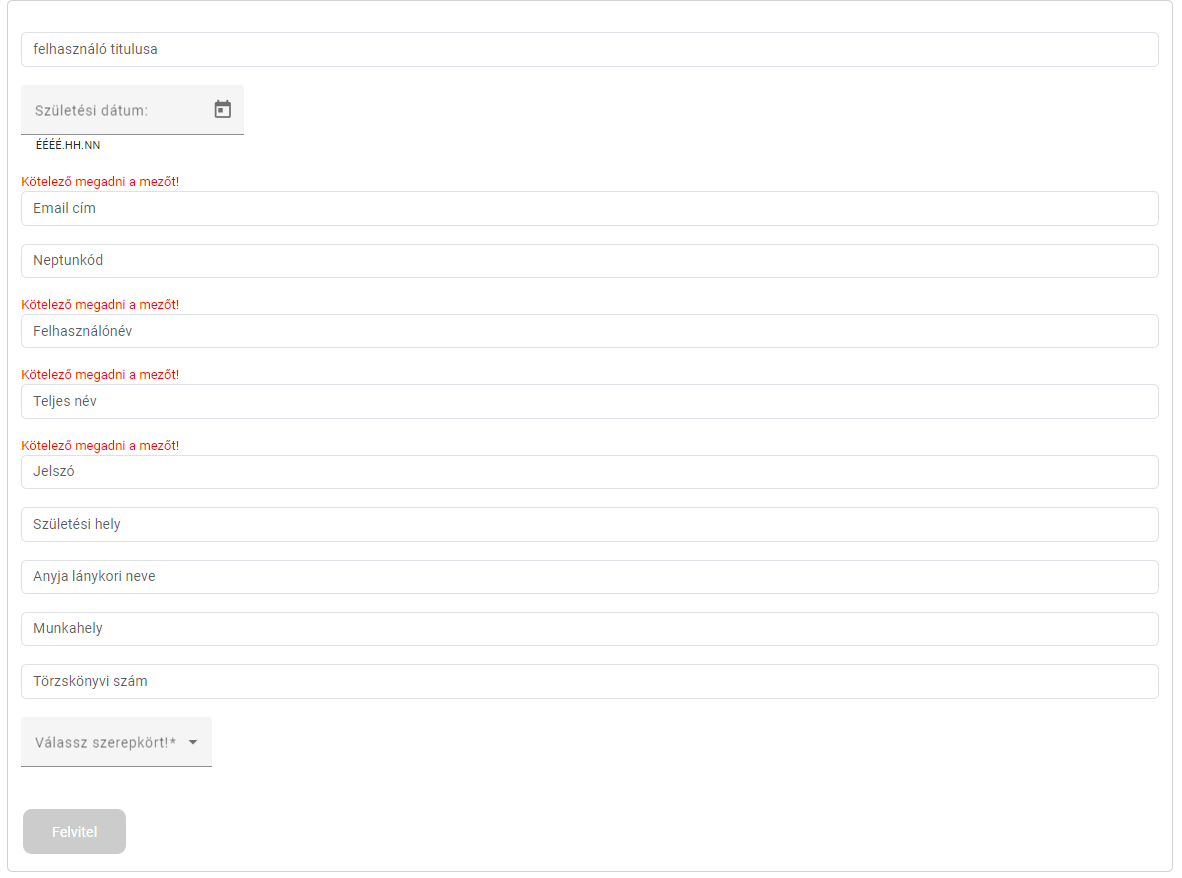
\includegraphics[width=\textwidth]{images/addUsers.png}
\caption{Felhasználó felvitele}
\label{fig:addUsers}
\end{figure}



\Section{Bírálat írása}

A bírálat írására szolgáló oldalon lehetősége van a témavezetőnek és bírálónak részletesen kifejteni a bírálatot a kiválasztott hallgatóhoz és szakdolgozathoz. A felhasználótól függően, aki éppen be van jelentkezve az alkalmazásba, választhatunk egy hallgatót a legördülő listából, aki az adott felhasználóhoz tartozik. Ezt követően a bírálatot részletesen megfogalmazhatjuk egy textarea mezőben. A bírálat osztályzatát is megadhatjuk. Végül, a felhasználó lehetőséget kap arra is, hogy megjelölje, hol készítette el a bírálatot.


\begin{figure}[h]
\centering
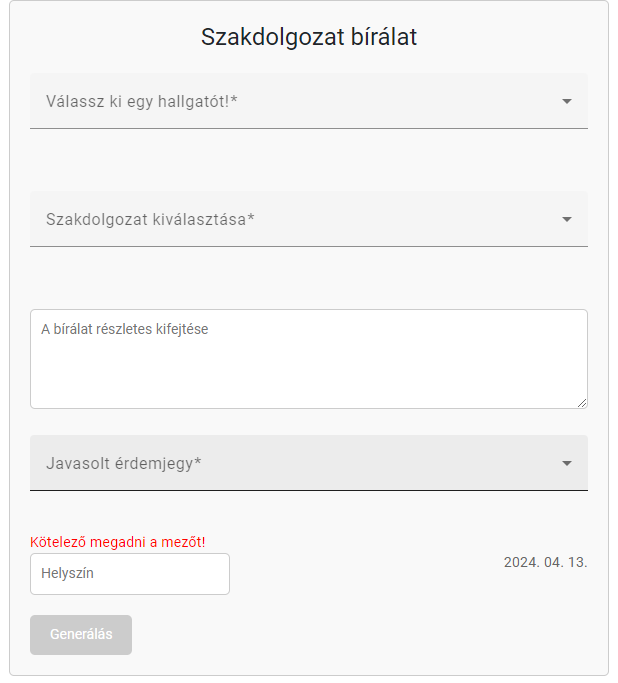
\includegraphics[scale=0.5]{images/Review.png}
\caption{Szakdolgozat bírálata}
\label{fig:Review}
\end{figure}

\newpage

\Section{Report status}

Az oldalon a szakdolgozatok bírálatának nyomon követése egy táblázatos elrendezésben valósult meg. Az oldalt három részre osztottam: a beadott szakdolgozatokra, a folyamatban lévő bírálatokra és a befejezett bírálatokra. Minden rész egy összecsukható listával rendelkezik, ami könnyű navigációt tesz lehetővé.\\
\\
A "Beadott szakdolgozatok" részben láthatóak a dolgozatok, valamint az azokhoz kapcsolódó hallgatók, témavezetők és bírálók. A szakdolgozathoz tartozó fájlokat is letölthetjük innen. Ezenkívül az alatta lévő táblázat a bíráló felkérésére lett létrehozva. Egy felugró ablakban választhatunk ki egy bírálót az adott szakdolgozathoz.\\
\begin{figure}[h]
\centering
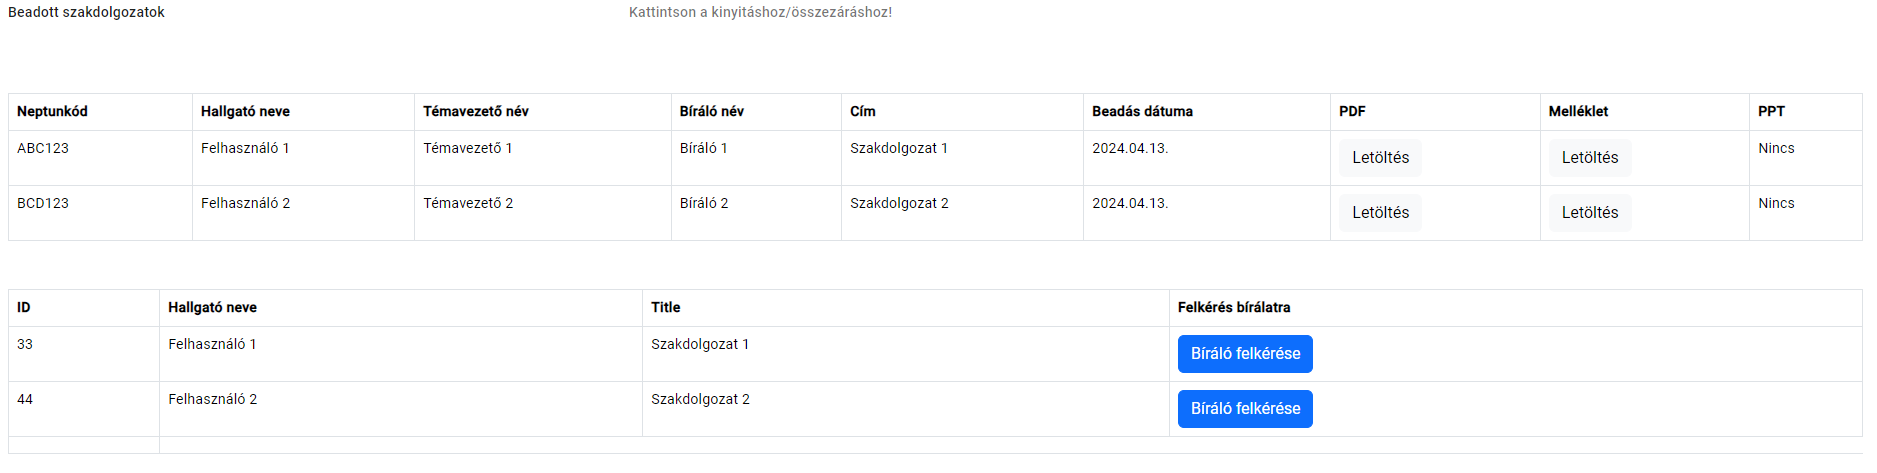
\includegraphics[width=\textwidth]{images/Report_status1.png}
\caption{Beadott szakdolgozatok}
\label{fig:Report_status1}
\end{figure}
\\A "Folyamatban lévő bírálatok" részben a bíráló neve automatikusan megjelenik, miután kiválasztottuk. A táblázat ugyanazokat az információkat tartalmazza, mint a "Beadott szakdolgozatok" esetében.\\
\begin{figure}[h]
\centering
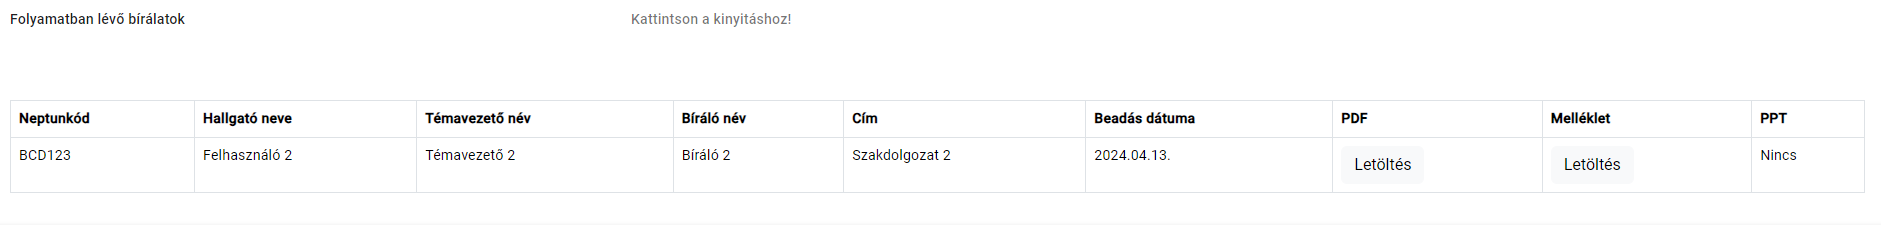
\includegraphics[width=\textwidth]{images/Report_status2.png}
\caption{Folyamatban lévő bírálatok}
\label{fig:Report_status2}
\end{figure}
\\Miután a bírálat befejeződött a témavezető és a bíráló részéről, a "Befejezett bírálatok" táblázathoz kerülünk, ahol lehetőségünk van a bírálatok letöltésére és azok elküldésére e-mailben a hallgatónak. Ez az elrendezés egyszerűsíti és átláthatóvá teszi a bírálatok kezelését és nyomon követését.
\begin{figure}[h]
\centering
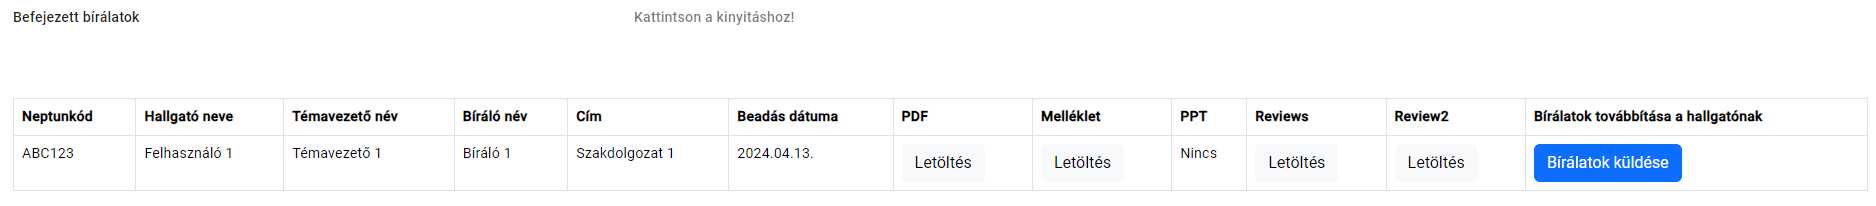
\includegraphics[width=\textwidth]{images/Report_status3.png}
\caption{Befejezett bírálatok}
\label{fig:Report_status3}
\end{figure}

